% Draft generated by Claude (2026-11-08) at the team's request; English translation of docs/pl/preprint/main.tex.
% To be rewritten by the team in their own words. Disclose AI use in the preprint. Experiment references (E##) are in comments only.
\documentclass[10pt,a4paper]{article}
\usepackage{iftex}
\ifXeTeX
  \usepackage{fontspec}
\else
  \usepackage[T1]{fontenc}
  \usepackage[utf8]{inputenc}
  \usepackage{lmodern}
\fi
\usepackage[english]{babel}
\usepackage[margin=2.2cm]{geometry}
\usepackage[table]{xcolor}
\usepackage{graphicx,booktabs,amsmath,enumitem,microtype}
\usepackage[hidelinks]{hyperref}
\usepackage[most]{tcolorbox}
\usepackage[font=small,labelfont=bf]{caption}
\usepackage[section]{placeins}
\newcommand{\capdet}[1]{\par\footnotesize\color{black!75}#1}
\setlist{nosep,leftmargin=1.4em}
\newcommand{\x}[1]{$\times$#1}
\newcommand{\todo}[1]{\textcolor{red!70!black}{\textbf{TODO:} #1}}

\title{Estimating hidden post views from reactions:\\transferring a model across platforms}
\author{AMC project team, Wroc{\l}aw University of Science and Technology}
\date{draft, \today}

\begin{document}
\maketitle


% ----------------------------------------------------------------

\section{Introduction}

Media monitoring companies such as Brand24 report to their clients how many people may have seen a mention of their
brand. The simplest reach measure, the view count, is often not visible: platforms limit what they show publicly, and
the scope of this data differs between platforms and post formats and changes over time. In practice reach is therefore
approximated by a fixed multiple of followers or reactions, which says nothing about how wrong it may be.

Predicting content popularity is widely studied~\cite{tatar2014}, also across services: Shulman et
al.~\cite{shulman2016} transfer a model between music, book, photo and link datasets, and Roy
et al.~\cite{roy2013} transfer knowledge from Twitter to YouTube videos. These works, however, predict future popularity
and have popularity data from the target platform on which the model is trained or calibrated. Our task is different:
we estimate current views from visible reactions on a platform from which the model gets not a single view count in
training. We collect views from that platform separately and use them only for evaluation. We found no work that tests
transferring a view model across platforms in this way.

We ask whether the views of a Facebook or Instagram post can be estimated from its reactions by a model trained only on
other platforms, and with what uncertainty. Our contributions:
\begin{itemize}
  \item a model trained only on X and YouTube estimates the views of Facebook videos with a typical error of \x{2.4}
        and of Instagram reels with \x{2.72}, almost as well as a model trained on the target platform itself;
  \item we show when this transfer works (reactions read together with views) and when it fails;
  \item we give an uncertainty interval for every post, valid also when data are missing;
  \item we show applications: a breakout alert, a brand ranking and media value.
\end{itemize}

\section{Data}

We use 12\,500 mentions of 348 brands from five platforms, provided by Brand24 (2\,500 per platform; 85\% were
published between April and August 2026, and 85\% are in English). For TikTok, YouTube and X the views are in the export.
For Facebook and Instagram they are not, so we read them ourselves, together with reactions from the same moment: 402
videos from 20 brands on Facebook and 642 reels from 11 brands on Instagram. Ordinary posts on these platforms have no
view counter, so the results apply only to videos and reels. Mention type and sentiment were labelled by language models
and then checked and corrected by a team member.

\begin{table}[!htb]
\centering\small
\caption{Data by platform.}
\label{tab:data}
\begin{tabular}{lrrlrrr}
\toprule
Platform & Brands & Authors & Source of views & Posts with views & Median views & Views per like \\
\midrule
TikTok    & 266 & 2\,411 & Brand24 export       & 2\,491 & 729    & 25 \\
YouTube   & 273 & 2\,041 & Brand24 export       & 2\,441 & 433    & 26 \\
X         & 252 & 1\,658 & Brand24 export       & 1\,803 & 27     & 22 \\
Facebook  & 20  & $\geq$182\textsuperscript{a} & own read (videos) & 402    & 1\,413 & 35 \\
Instagram & 11  & ?\textsuperscript{b} & own read (reels) & 642    & 504    & 53 \\
\bottomrule
\end{tabular}
\par\footnotesize a: author known for 74\% of videos. b: author known for only 11\% of reels (59 authors among 72).\par
\end{table}

\begin{figure}[!htb]
\centering
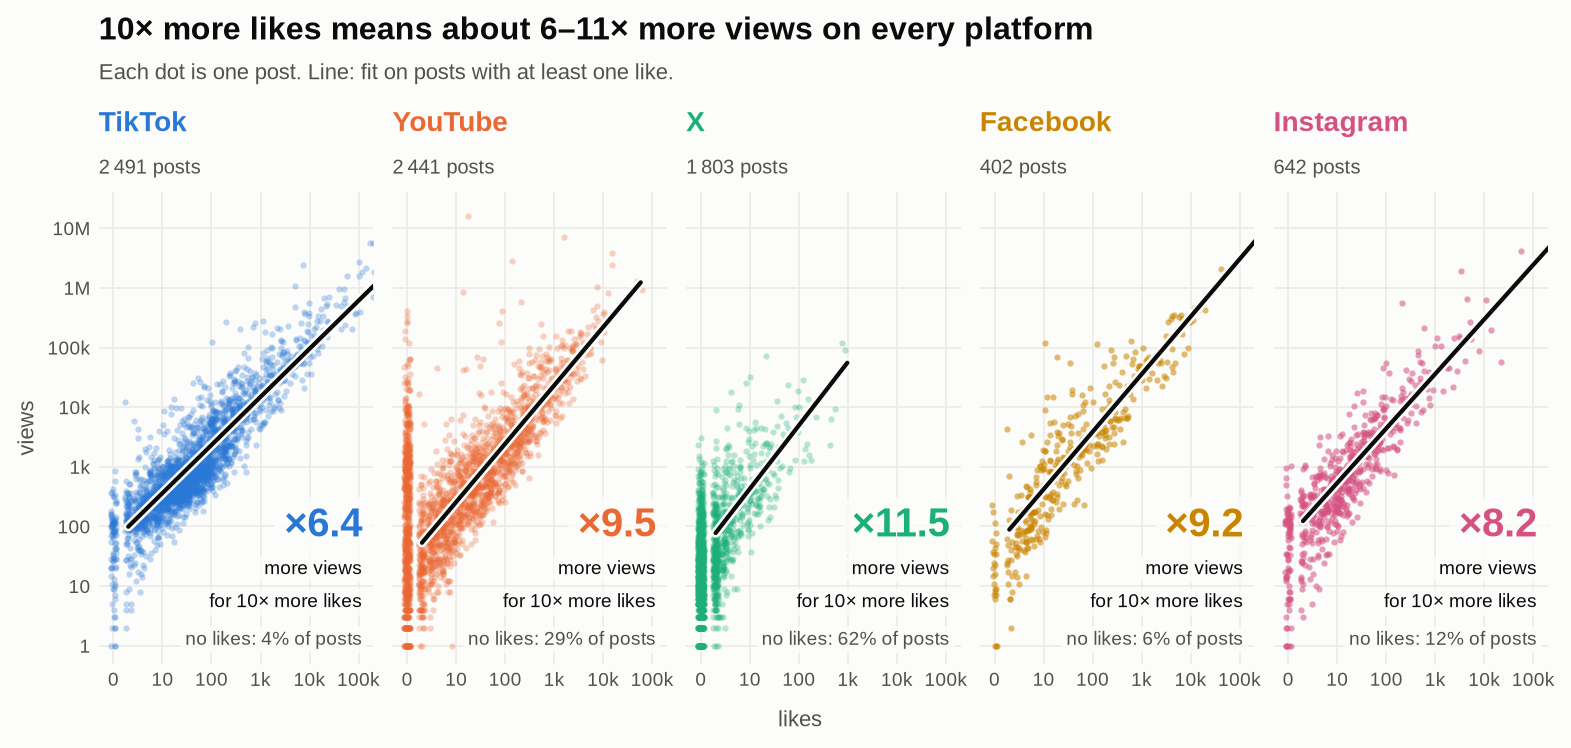
\includegraphics[width=\textwidth]{fig/data_overview_en.png}
\caption{Views versus likes, separately for each platform.
\capdet{Both axes on a log scale; posts without likes at zero. Line: fit on posts with at least one like; number: how
many times more views a post with 10 times more likes has. TikTok, YouTube, X: Brand24 export; Facebook (videos),
Instagram (reels): our read.}}
\label{fig:data}
\end{figure}

\section{Method}\label{sec:met}

We predict $y=\log_{10}(\text{views})$. We report the error as MAE on this scale and as the factor
$10^{\text{MAE}}$ (MAE 0.30 $\approx$ \x{2}). The final model is evaluated with five-fold cross-validation in which the
same brand, the same author or an identical text never appears in both training and test: one author may write about
several brands (1--9\% of posts), and the same text is sometimes pasted on different accounts. Every evaluation is thus
on a brand and an author the model has not seen. Confidence intervals come from a bootstrap over brands. Method
comparisons (Section~\ref{sec:nie}, same platform only) use a simpler split by brand alone; the stricter split changes
the error by at most 0.002 on TikTok and YouTube and by 0.012 on X, equally for all methods.
\begin{tcolorbox}[colback=black!3,colframe=black!25,boxrule=.4pt,left=4pt,right=4pt,top=2pt,bottom=2pt]\small
\textbf{Two scenarios, marked in every figure.} \emph{Same platform}: the model is trained on posts from the given
platform (TikTok, YouTube, X) and evaluated on brands and authors it has not seen. \emph{Out of platform}: the model sees
not a single post from the target platform in training (Facebook, Instagram, Stack Exchange; in Table~\ref{tab:combos}
each platform in turn), and its views are used only for evaluation.
\end{tcolorbox}

On TikTok, YouTube and X we use CatBoost~\cite{catboost} on followers, reactions and missingness flags. For the transfer
to Facebook and Instagram we use ridge regression on $\log(1+\text{likes})$ and $\log(1+\text{comments})$, the two
fields every platform has, trained on X and YouTube together; with the target platform left out it transfers better
than CatBoost. Per-post 50\% and 90\% intervals come from conformalized quantile regression~\cite{romano2019}.
% E55, E222 (results_a on brand+author+text split). E114, E124, E61/E131 (ridge > CatBoost with platform left out), E118, E137.

\section{Results}\label{sec:wyniki}

\paragraph{Main result.} Fig.~\ref{fig:main} shows both scenarios. On TikTok, YouTube and X, where the model is trained
on the same platform, the typical error is \x{1.9}, \x{2.9} and \x{3.0}. On Facebook and Instagram the model has not
seen a single post from these platforms, and its error is \x{2.43} (confidence interval \x{2.05}--\x{3.03}) and
\x{2.72} (\x{2.49}--\x{3.05}). On Facebook this equals the same model trained on the target platform itself
(\x{2.42}); on Instagram it is slightly worse than training on Instagram alone (\x{2.41}; 72\% of reels are
underestimated), so the relation between reactions and views transfers across platforms almost without loss. The
ordering of posts is preserved very well (Spearman 0.91 and 0.86).
% results_a/results_b_numbers.json; CI MAE 0.312-0.482 and 0.396-0.484.

\begin{figure}[!htb]
\centering
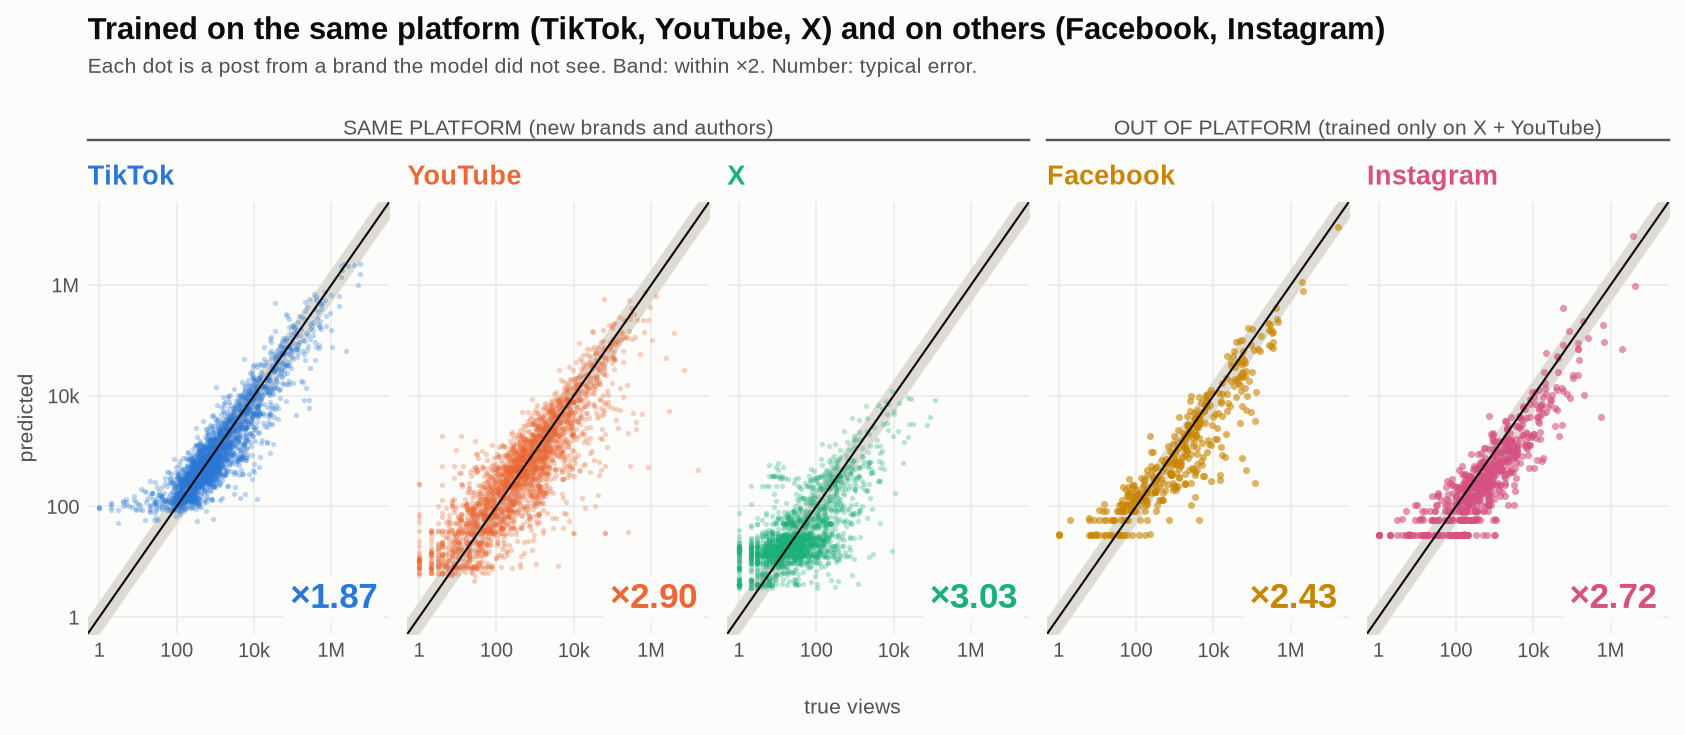
\includegraphics[width=\textwidth]{fig/preprint_main_en.png}
\caption{Estimated versus true views.
\capdet{Each dot is one post, estimated by a model that has not seen its brand (brand-grouped cross-validation).
TikTok, YouTube, X: CatBoost on followers, reactions and missingness flags, trained on the same platform; truth from the
Brand24 export. Facebook (402 videos, 20 brands), Instagram (642 reels, 11 brands): ridge on $\log$ likes and comments
trained only on X and YouTube; truth from our read. Grey band: estimate within \x{2}. Number: typical error
$10^{\text{MAE}}$.}}
\label{fig:main}
\end{figure}

\paragraph{Who is estimated badly.} On every platform, also after transfer, the model overestimates posts with few views
(about \x{2} below 100 views) and underestimates large ones (Fig.~\ref{fig:size}). This is the usual regression to the
mean: reactions do not separate a post that broke out from an ordinary one well. It is strongest on X, where posts above
10\,000 views are underestimated more than tenfold; after transfer, Instagram underestimates large reels by about \x{3}.

\begin{figure}[!htb]
\centering
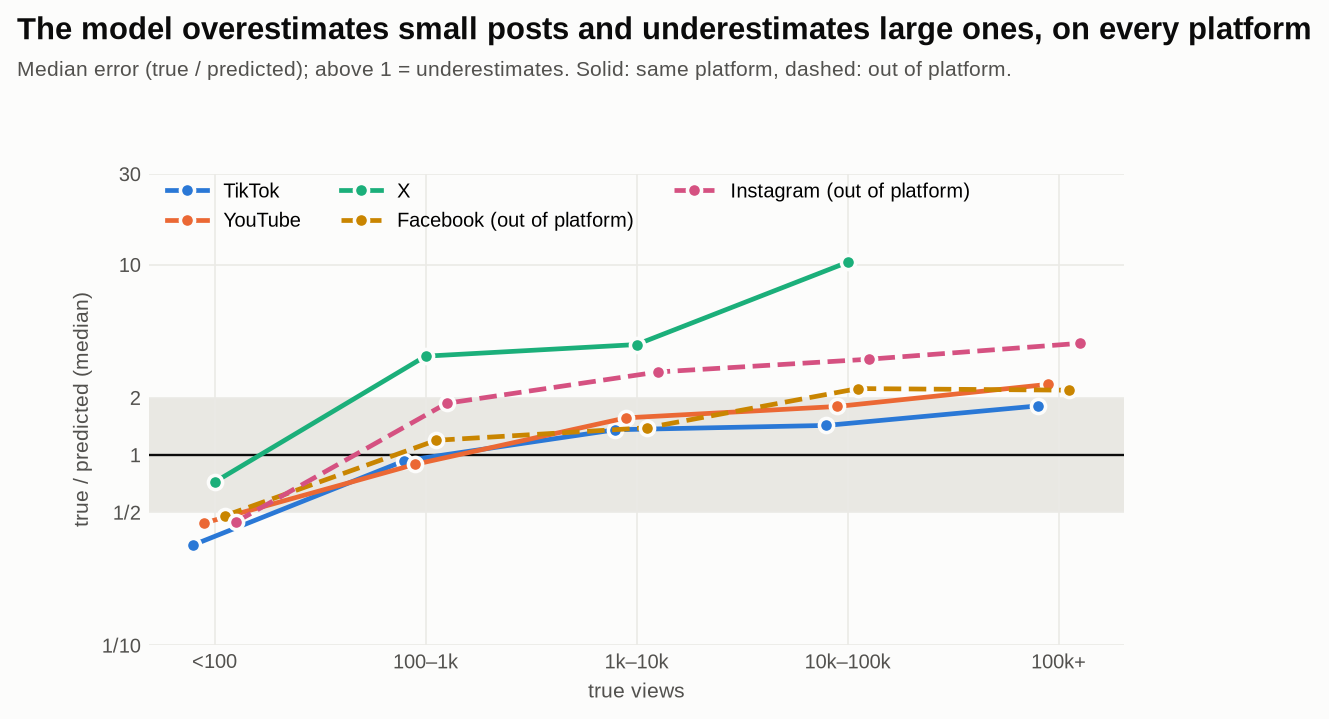
\includegraphics[width=.78\textwidth]{fig/preprint_size_en.png}
\caption{Error by post size.
\capdet{Median ratio of true to estimated views in bins of true views (bins with at least 10 posts shown). Above 1: the
model underestimates. Grey band: within \x{2}. Solid line: same platform, dashed: out of platform. Models as in
Fig.~\ref{fig:main}.}}
\label{fig:size}
\end{figure}


\paragraph{Intervals.} The 90\% interval covers 87--91\% of posts on TikTok, YouTube and X, also on months outside
training (0.90--0.93). On Facebook it covers 93\% of videos from accounts below one million followers, but only 80--86\%
for the largest accounts. If instead of a number we report one of three ranges (<1\,000, 1\,000--10\,000, >10\,000), we
are right for 78--82\% of posts on TikTok, YouTube, Facebook and Instagram.
% E118, E142, E123, E151, E199.

\section{Transfer across platforms}\label{sec:transfer}

\paragraph{Where we know the truth.} We have true views on all five platforms (Table~\ref{tab:data}): on TikTok, YouTube
and X from the Brand24 export, on Facebook (videos) and Instagram (reels) from our read, together with likes and comments
from the same moment. This lets us treat each platform as ``hidden'': we train the model on the others and test it on
this one. We use only the two fields every platform has, likes and comments, and plain ridge regression, because with
the target platform left out it transfers better than CatBoost. In practice Facebook and Instagram matter, since
monitoring data have no views there; the other platforms show how general the result is.

\paragraph{All combinations.} Table~\ref{tab:combos} shows the error for each of the 31 sets of training platforms.
Three things stand out. First, Facebook and Instagram can be estimated from almost any set with an error of
\x{2.4}--\x{3.1}, close to a model trained on them alone (\x{2.4}); training on X alone is the worst. Second, X is an
exception in both directions: a model trained on X has an error of \x{5.5} on YouTube, and no set gets below \x{3.6} on
X, against \x{3.3} when trained on X. On X most posts have zero or one like (Fig.~\ref{fig:data}), so the relation of
views to likes looks different there. Third, YouTube is hard even for a model trained on it (\x{4.1} for ridge against
\x{2.8} for CatBoost), because many videos have views without any reactions. More platforms in training do not always
help: what matters is which platforms are in the set and in what proportions.
% E201 (train_combos_numbers.json, pooled). Best: TT from YT 2.0; YT from TT+FB 4.06; X from FB 3.60; FB from YT+X+IG 2.39; IG from FB 2.47.

\begin{table}[!htb]
\centering\scriptsize
\setlength{\tabcolsep}{5pt}\renewcommand{\arraystretch}{1.05}
\caption{Typical error (\x{}) of the regression on likes and comments with different training platforms.
\capdet{Ridge on $\log$ likes and comments, posts from the training platforms pooled into one set. Row: platforms in
training (TT TikTok, YT YouTube, X, FB Facebook, IG Instagram): single ones, X + YouTube (the main set), TikTok + YouTube + X
and all sets of four platforms; the full table of 30 sets is in the repository. Column: test platform, absent from training. First row:
the same ridge trained on the test platform itself (brand-grouped CV), not the CatBoost of Fig.~\ref{fig:main}. Bold:
best result in the column among those shown. Darker: larger error.}}
\label{tab:combos}
\begin{tabular}{l|ccccc}
\toprule
Trained on & TikTok & YouTube & X & Facebook & Instagram \\
\midrule
\textit{ridge, same platform} & \cellcolor[HTML]{DDEBFC}2.0 & \cellcolor[HTML]{5A95DF}4.1 & \cellcolor[HTML]{A3C8F2}3.3 & \cellcolor[HTML]{DDEBFC}2.4 & \cellcolor[HTML]{DDEBFC}2.4 \\ \midrule
YT & \cellcolor[HTML]{DDEBFC}\textbf{2.0} & \cellcolor[HTML]{EEEDEA}{\color{black!35}train} & \cellcolor[HTML]{3779CF}\textcolor{white}{4.6} & \cellcolor[HTML]{C3DCF8}2.7 & \cellcolor[HTML]{C3DCF8}2.6 \\
FB & \cellcolor[HTML]{DDEBFC}2.3 & \cellcolor[HTML]{3779CF}\textcolor{white}{4.3} & \cellcolor[HTML]{7FB0EA}\textbf{3.6} & \cellcolor[HTML]{EEEDEA}{\color{black!35}train} & \cellcolor[HTML]{C3DCF8}\textbf{2.5} \\
IG & \cellcolor[HTML]{C3DCF8}2.5 & \cellcolor[HTML]{3779CF}\textcolor{white}{4.5} & \cellcolor[HTML]{5A95DF}4.1 & \cellcolor[HTML]{C3DCF8}2.5 & \cellcolor[HTML]{EEEDEA}{\color{black!35}train} \\
TT & \cellcolor[HTML]{EEEDEA}{\color{black!35}train} & \cellcolor[HTML]{5A95DF}\textbf{4.1} & \cellcolor[HTML]{5A95DF}4.1 & \cellcolor[HTML]{C3DCF8}2.6 & \cellcolor[HTML]{C3DCF8}2.6 \\
X & \cellcolor[HTML]{7FB0EA}3.4 & \cellcolor[HTML]{184A8C}\textcolor{white}{5.5} & \cellcolor[HTML]{EEEDEA}{\color{black!35}train} & \cellcolor[HTML]{A3C8F2}3.1 & \cellcolor[HTML]{C3DCF8}2.7 \\
\midrule
YT + X & \cellcolor[HTML]{DDEBFC}2.1 & \cellcolor[HTML]{EEEDEA}{\color{black!35}train} & \cellcolor[HTML]{EEEDEA}{\color{black!35}train} & \cellcolor[HTML]{DDEBFC}\textbf{2.4} & \cellcolor[HTML]{C3DCF8}2.7 \\
\midrule
TT + YT + X & \cellcolor[HTML]{EEEDEA}{\color{black!35}train} & \cellcolor[HTML]{EEEDEA}{\color{black!35}train} & \cellcolor[HTML]{EEEDEA}{\color{black!35}train} & \cellcolor[HTML]{C3DCF8}2.5 & \cellcolor[HTML]{C3DCF8}2.7 \\
\midrule
YT + X + FB + IG & \cellcolor[HTML]{DDEBFC}2.1 & \cellcolor[HTML]{EEEDEA}{\color{black!35}train} & \cellcolor[HTML]{EEEDEA}{\color{black!35}train} & \cellcolor[HTML]{EEEDEA}{\color{black!35}train} & \cellcolor[HTML]{EEEDEA}{\color{black!35}train} \\
TT + YT + X + IG & \cellcolor[HTML]{EEEDEA}{\color{black!35}train} & \cellcolor[HTML]{EEEDEA}{\color{black!35}train} & \cellcolor[HTML]{EEEDEA}{\color{black!35}train} & \cellcolor[HTML]{C3DCF8}2.5 & \cellcolor[HTML]{EEEDEA}{\color{black!35}train} \\
TT + YT + X + FB & \cellcolor[HTML]{EEEDEA}{\color{black!35}train} & \cellcolor[HTML]{EEEDEA}{\color{black!35}train} & \cellcolor[HTML]{EEEDEA}{\color{black!35}train} & \cellcolor[HTML]{EEEDEA}{\color{black!35}train} & \cellcolor[HTML]{C3DCF8}2.7 \\
TT + X + FB + IG & \cellcolor[HTML]{EEEDEA}{\color{black!35}train} & \cellcolor[HTML]{5A95DF}4.1 & \cellcolor[HTML]{EEEDEA}{\color{black!35}train} & \cellcolor[HTML]{EEEDEA}{\color{black!35}train} & \cellcolor[HTML]{EEEDEA}{\color{black!35}train} \\
TT + YT + FB + IG & \cellcolor[HTML]{EEEDEA}{\color{black!35}train} & \cellcolor[HTML]{EEEDEA}{\color{black!35}train} & \cellcolor[HTML]{3779CF}\textcolor{white}{4.4} & \cellcolor[HTML]{EEEDEA}{\color{black!35}train} & \cellcolor[HTML]{EEEDEA}{\color{black!35}train} \\
\bottomrule
\end{tabular}
\end{table}


\paragraph{Three ranges instead of a number.} A report often only needs to say whether a post had fewer than a thousand,
one to ten thousand, or more than ten thousand views. Fig.~\ref{fig:bins} shows this out of platform for each of the five
platforms: a model trained on the other four, without any post from the target platform. Accuracy is 78--81\%, but the
ranges differ greatly in size, so balanced accuracy (mean recall over ranges) matters more: 78\% on TikTok, 76\% on
Facebook, 70\% on YouTube and 65\% on Instagram, against 33\% for guessing; macro F1 0.70--0.78. We are off by two ranges
for 0.2--1.9\% of posts. The middle range (1--10 thousand views, recall 50--73\%) is the weakest; its posts are usually
underestimated by one range.

X looks different: accuracy 96\%, but balanced accuracy only 46\% and macro F1 0.52. On X 95\% of posts have fewer than a
thousand views (median 27), so a model that almost always says ``below a thousand'' gets high accuracy for free. Of 98
posts above a thousand it gets only 23 right. There are two reasons. First, 62\% of posts on X have no like at all, so
the model sees only a zero there and cannot tell a small post from a large one. Second, views in the X export are read
early and are about two times lower than in our re-read, and the same model has an error of 0.49 on re-read X instead
of 0.64 (E219). Large posts on X thus look small to the model.
% preprint_bins_numbers.json (ridge E201, other four); E204, E219.

\begin{figure}[!htb]
\centering
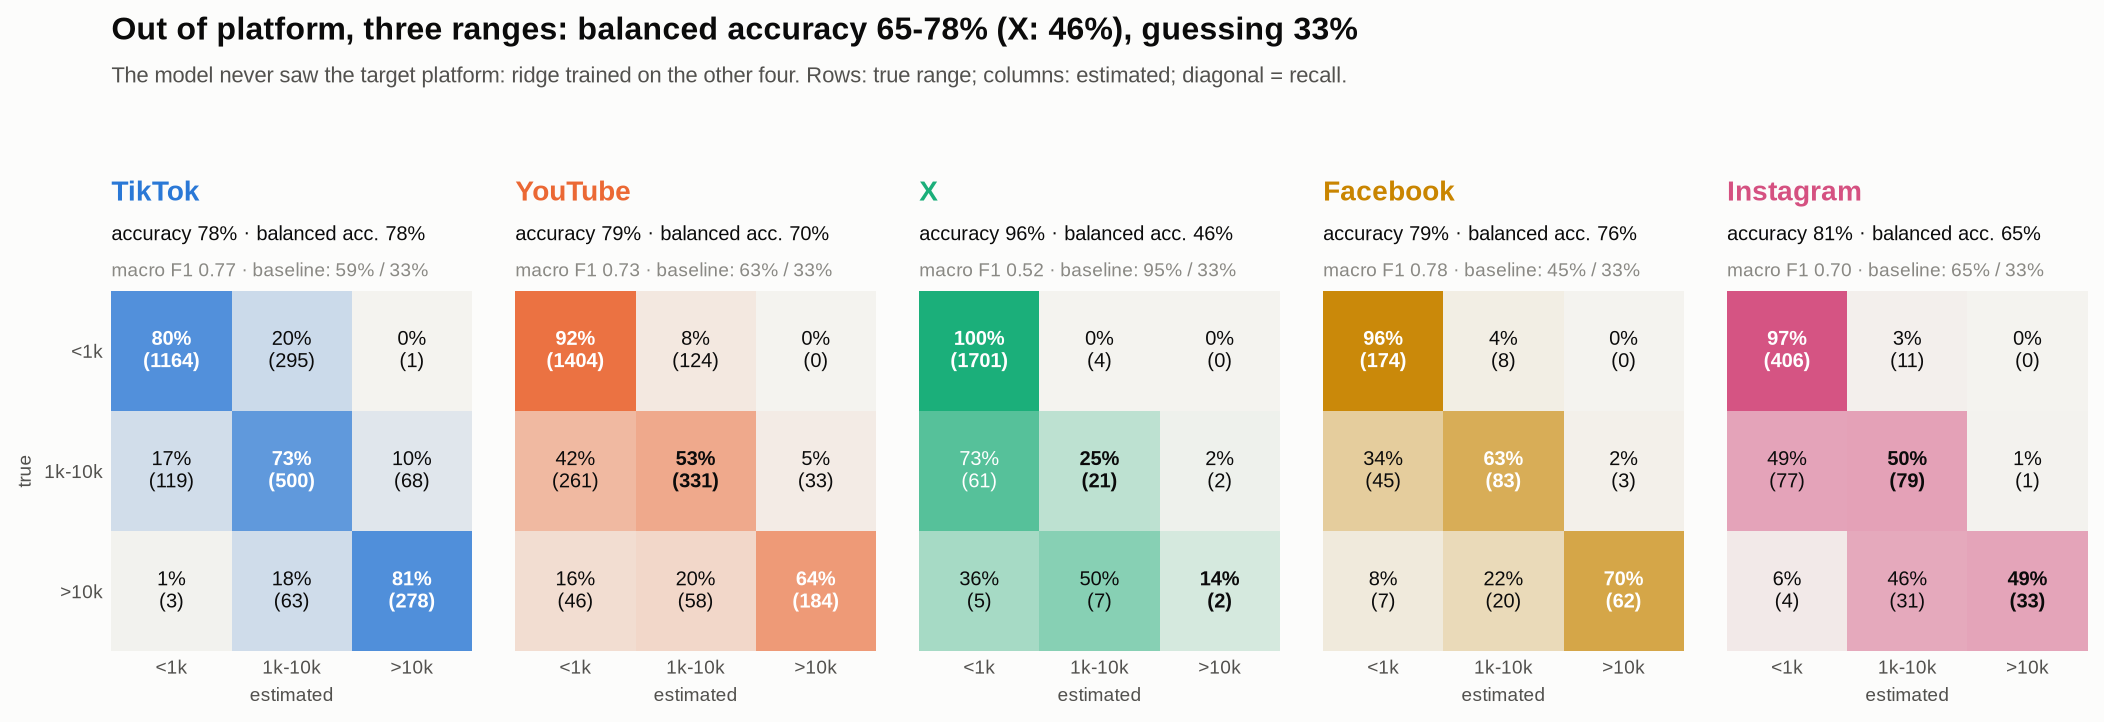
\includegraphics[width=\textwidth]{fig/preprint_bins_en.png}
\caption{Out-of-platform estimate cut into three view ranges.
\capdet{For each platform, ridge on likes and comments trained on the other four (as in the last row of
Table~\ref{tab:combos}). Row: true range; column: estimated; in a cell: share of the row and number of posts; the
diagonal (bold) is the recall of the range. Above the table: accuracy, balanced accuracy (mean recall), macro F1; grey:
accuracy and balanced accuracy when always guessing the most frequent range.}}
\label{fig:bins}
\end{figure}

\paragraph{What the model needs.} The transfer works only with likes read together with views (Fig.~\ref{fig:needs}A).
Comments alone give \x{6.3}--\x{7.4}, and likes and comments from the export, read at a different moment than views,
\x{6.8}. On platforms with known views (Fig.~\ref{fig:needs}B) missing followers hardly hurt, while missing reactions
raise the error to \x{3.8}--\x{5.2}. For each pattern of available fields we train a separate model with its own
interval, so the 90\% interval covers 88--90\% of posts in every case; a model trained on full data and fed incomplete
data would cover only 46--83\%.
% E177, E176, results_b (comments only).

\begin{figure}[!htb]
\centering
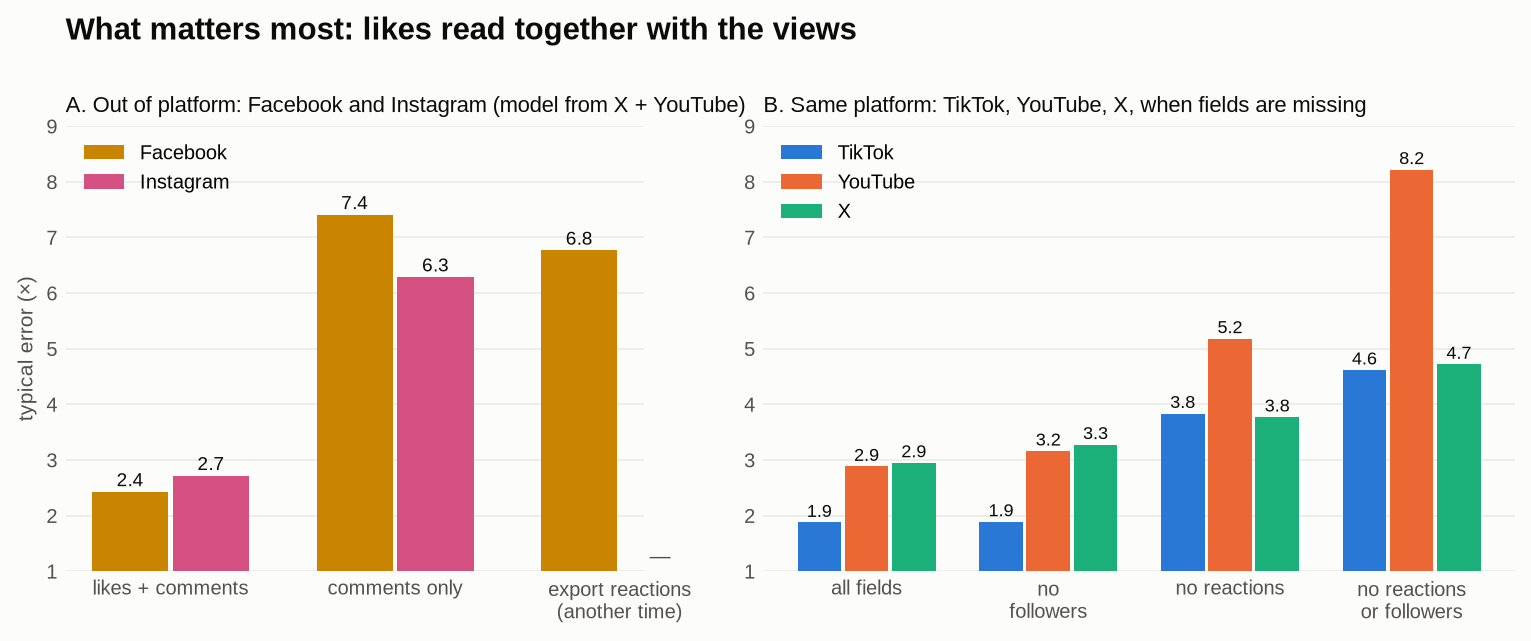
\includegraphics[width=\textwidth]{fig/preprint_needs_en.png}
\caption{Typical error with different inputs.
\capdet{A: Facebook and Instagram, ridge trained on X and YouTube. ``Likes + comments'': our fields read together with
views; ``comments only'': a model on comments alone; ``export reactions'': likes and comments from the Brand24 export,
read at a different moment than views (not available for Instagram). B: TikTok, YouTube, X, a separate CatBoost for each
pattern of available fields, brand-grouped validation. A: out of platform, B: same platform.}}
\label{fig:needs}
\end{figure}

\paragraph{Fresh source data.} Views in the export are read shortly after publication, and our Facebook and Instagram
reads several months later. When the same model is trained on re-read X and YouTube, with reactions from the same
moment, the error on Instagram drops from \x{2.72} to \x{2.41} (as much as a model trained on Instagram alone), and on
Facebook it stays at \x{2.44}. The underestimation of large posts and of brand totals roughly halves. Merely shifting
export views to a later age does not achieve this, so what matters is that views and reactions come from the same
moment. For the same reason X does badly as a test platform mainly because of stale labels: the same model has an error
of 0.64 on export X and 0.49 on re-read X. X posts without likes are not the cause here.
% E210, E211, E213, E218, E219. Main numbers in the text still on the Brand24 export.

\paragraph{A sixth platform.} To test the transfer outside social media, we fetched through the public API 538
questions from Stack Exchange sites (among others Stack Overflow, Super User, Android, Apple, Mechanics) about 48 brands
from our data, from the same period (April--August 2026). We treat an upvote as a like, and answers and comments as
comments; this mapping was fixed before evaluation. A model trained on X and YouTube has an error of \x{3.14} here, and
the same ridge trained on Stack Exchange alone \x{1.77}. The ordering of questions transfers equally well (Spearman 0.57
in both cases), but 96\% of questions are underestimated: question views accumulate over months and an upvote is not a
like, so the whole level is shifted. YouTube alone transfers best (\x{1.87}), X alone worst (\x{4.50}), as on Facebook
and Instagram.
% E225 (stackexchange_numbers.json).

\section{Comparison of methods}\label{sec:nie}

\paragraph{Model families.} Table~\ref{tab:models} compares models on the same inputs. After tuning, almost all
families give the same error: \x{1.85}--\x{1.92} on TikTok, \x{2.8}--\x{2.9} on YouTube and \x{2.9}--\x{3.1} on X.
Only the simple baselines (\x{4.6}--\x{8.8}) and linear regression and kNN on YouTube (\x{3.0}--\x{3.5}) are clearly
worse. The best single model is TabPFN v2, but it beats CatBoost by only 0.002--0.010, within the run-to-run noise, and
takes about 150 times longer. The graph network and a transformer reading the post as text are worse than CatBoost.

\paragraph{Why not an ensemble.} An ensemble combines the estimates of several models, e.g.\ by averaging them (``mean
of top 3'') or with a second-level model that learns how to weight the estimates of all families (``stack''). Errors of
different models partly cancel, so an ensemble is usually slightly better than each member. Here the stack improves the
result by 0.011--0.028 (\x{1.03}--\x{1.07}). We keep a single model for three reasons: (1) the gain is small against the
typical error of \x{1.9}--\x{3.0}; (2) a stack requires training and maintaining over a dozen models, while the
uncertainty intervals (CQR) and the transfer to other platforms are built on one model; (3) in the transfer the simplest
linear model wins anyway (Section~\ref{sec:met}), so complexity does not carry over to the main result.
% E11, E47 (TabPFN 136-176 s vs CatBoost 1 s), E54, E61/E131.

\begin{table}[!htb]
\centering\small
\caption{Comparison of model families: MAE on the $\log_{10}$ scale and typical error (\x{}).
\capdet{All models on followers, reactions and missingness flags, brand-grouped cross-validation. Tree, linear, kernel and MLP models after hyperparameter tuning (40 settings per fold, nested tuning). TabPFN, TabICL, GraphSAGE, transformer and stack come from separate runs on the same data; CatBoost in those runs stayed within 0.271--0.273 / 0.452--0.456 / 0.466--0.470, so differences below about 0.005 are within noise. Bold: best single model in the column. Ensembles shown for comparison only.}}
\label{tab:models}
\begin{tabular}{lccc}
\toprule
Model & TikTok & YouTube & X \\
\midrule
\multicolumn{4}{l}{\textit{Simple baselines}} \\
\quad platform median views & 0.663 (\x{4.60}) & 0.944 (\x{8.79}) & 0.667 (\x{4.65}) \\
\quad fixed multiple of followers & 0.919 (\x{8.30}) & 0.855 (\x{7.16}) & 0.879 (\x{7.57}) \\
\multicolumn{4}{l}{\textit{Linear and kernel models}} \\
\quad linear regression (ridge) & 0.277 (\x{1.89}) & 0.545 (\x{3.51}) & 0.487 (\x{3.07}) \\
\quad k nearest neighbours (kNN) & 0.283 (\x{1.92}) & 0.483 (\x{3.04}) & 0.490 (\x{3.09}) \\
\quad SVR with RBF kernel & 0.271 (\x{1.87}) & 0.463 (\x{2.90}) & 0.480 (\x{3.02}) \\
\multicolumn{4}{l}{\textit{Decision trees}} \\
\quad random forest & 0.275 (\x{1.88}) & 0.463 (\x{2.90}) & 0.473 (\x{2.97}) \\
\quad extra trees & 0.275 (\x{1.88}) & 0.459 (\x{2.88}) & 0.475 (\x{2.99}) \\
\quad gradient boosting (scikit-learn) & 0.276 (\x{1.89}) & 0.453 (\x{2.84}) & 0.474 (\x{2.98}) \\
\quad LightGBM & 0.275 (\x{1.88}) & 0.457 (\x{2.86}) & 0.475 (\x{2.99}) \\
\quad XGBoost & 0.273 (\x{1.87}) & 0.450 (\x{2.82}) & 0.467 (\x{2.93}) \\
\quad CatBoost (final model) & 0.272 (\x{1.87}) & 0.452 (\x{2.83}) & 0.470 (\x{2.95}) \\
\multicolumn{4}{l}{\textit{Neural networks}} \\
\quad multilayer perceptron (MLP) & 0.276 (\x{1.89}) & 0.454 (\x{2.84}) & 0.477 (\x{3.00}) \\
\quad GraphSAGE graph network (similar-text graph) & 0.279 (\x{1.90}) & 0.467 (\x{2.93}) & 0.474 (\x{2.98}) \\
\quad fine-tuned transformer (row as text) & 0.289 (\x{1.95}) & 0.454 (\x{2.84}) & 0.490 (\x{3.09}) \\
\multicolumn{4}{l}{\textit{Pretrained tabular models}} \\
\quad TabPFN v2 & \textbf{0.268 (\x{1.85})} & \textbf{0.443 (\x{2.77})} & \textbf{0.465 (\x{2.92})} \\
\quad TabICL & 0.272 (\x{1.87}) & 0.445 (\x{2.79}) & 0.466 (\x{2.92}) \\
\midrule
\multicolumn{4}{l}{\textit{Ensembles (for comparison)}} \\
\quad mean of top 3 families & 0.270 (\x{1.86}) & 0.446 (\x{2.79}) & 0.469 (\x{2.94}) \\
\quad stack of all families & 0.260 (\x{1.82}) & 0.425 (\x{2.66}) & 0.441 (\x{2.76}) \\
\bottomrule
\end{tabular}
\end{table}
% E11 (tuning_numbers.json), E47, E53, E54, E65; blend = tuning_numbers.json blend.

\paragraph{Extra data.} We also tested more than twenty additional signal sources (Fig.~\ref{fig:methods}): text (from
TF-IDF to sentence embeddings), AI labels, author and brand graphs, and external brand data. None changes the error by
more than \x{1.04}, and most by less than \x{1.02} or make it worse. Text helps slightly on YouTube and X, graphs and
external data hurt. On Facebook text worsens the transfer (MAE 0.385 $\to$ 0.436). Author history is described
separately below.
% E50, E65, E127, E170-E175, ablation; E100 (FB text); E68/E70 (author).

\paragraph{More data without new labels.} We also tested methods that add data or learn its structure without views.
Synthetic large posts (SMOTER/SMOGN) reduce the underestimation of the most popular tenth of posts, but only by
stretching the scale of the estimates, and raise the error by 0.006--0.019. Random perturbation along the trend and mixup
do not let CatBoost or an MLP transfer as well as ridge (they stay 0.014--0.062 behind on each of the five platforms).
A representation learned without labels (denoising autoencoder, SCARF) changes the error by at most 0.005, and
pseudo-labels for posts without views by at most 0.008. The final model therefore stays without augmentation.
% E214 smoter_tail, E215 aug_transfer, E216 ssl_repr, E217 pseudo_label.

\begin{figure}[!htb]
\centering
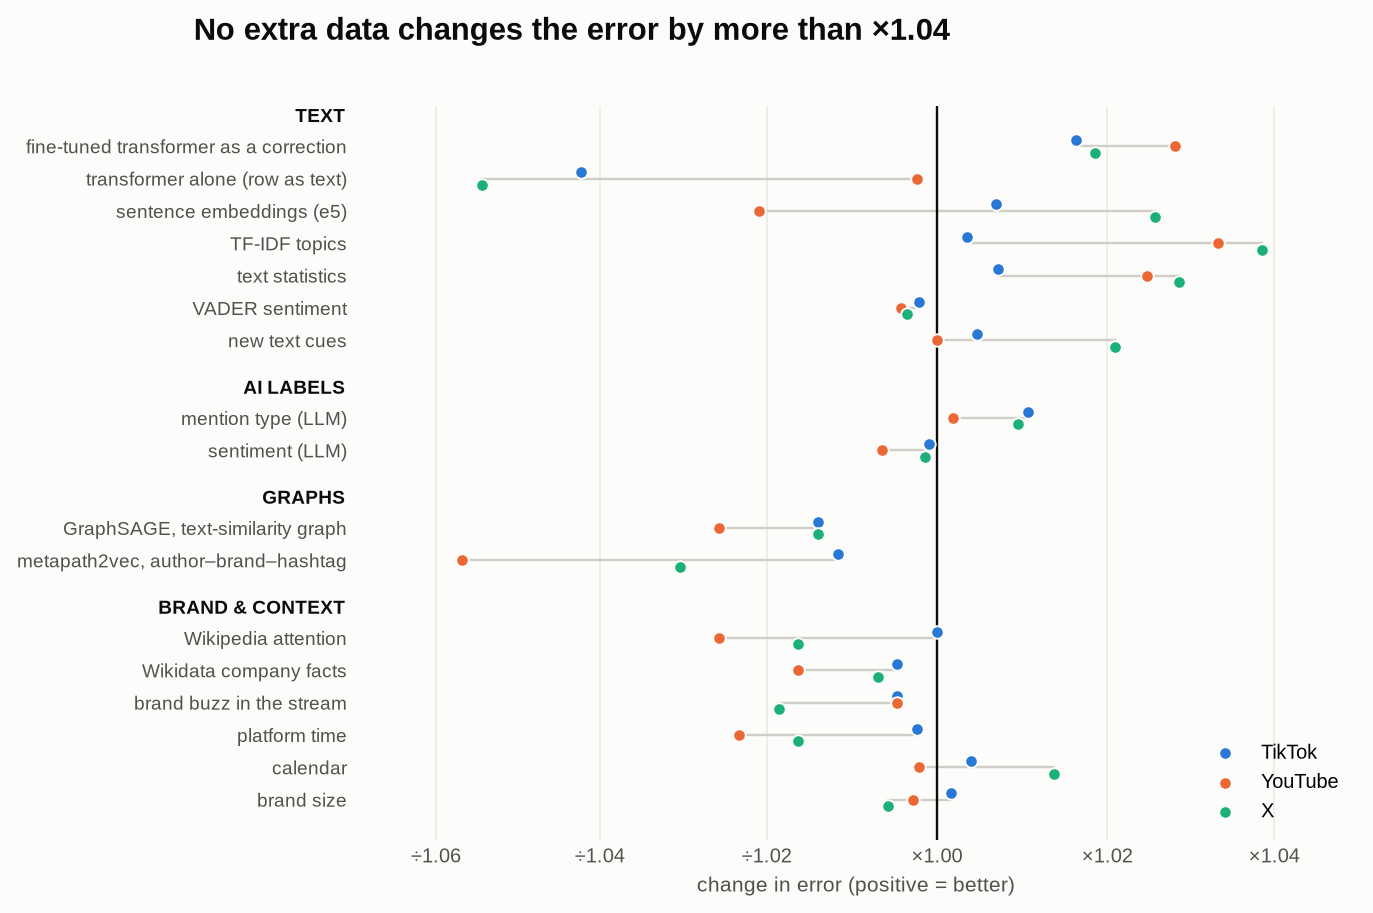
\includegraphics[width=.85\textwidth]{fig/preprint_methods_en.png}
\caption{Extra data and features.
\capdet{Change in typical error relative to the final model (transformer as correction, embeddings, graphs, external
data) or relative to the model on followers and reactions (TF-IDF, text statistics, VADER, AI labels, calendar, brand
size). Right: better, left: worse; \x{1.02} is a change in MAE of about 0.01. \emph{Transformer as correction}: a
fine-tuned language model predicts the CatBoost error from the post text. \emph{e5 embeddings}: a multilingual sentence
model. \emph{LLM labels}: mention type and sentiment from a language model. \emph{GraphSAGE}: a graph network on the
similar-text graph; \emph{metapath2vec}: embeddings of the author--brand--hashtag graph. \emph{Wikipedia, Wikidata}:
interest in the brand and company data. All with brand-grouped validation.}}
\label{fig:methods}
\end{figure}

\paragraph{Author history.} The only signal that clearly helps is author history. The same author gets a similar number
of views on successive posts, regardless of reactions: the correlation of the view surplus (truth minus estimate)
between an author's first and later posts is 0.68--0.70 on all three platforms, and authors in the top third get 4--9
times more views than those in the bottom third at the same estimate. We use this simply: to the estimate of a new post
we add the mean surplus of the author's earlier posts, shrunk towards zero when there are few posts (sum of surpluses
divided by the number of posts plus a constant tuned on other brands). On posts by authors with history the error drops
from 0.37 to 0.26 on TikTok, from 0.50 to 0.35 on YouTube and from 0.53 to 0.43 on X (\x{1.3}--\x{1.4}); most of the
gain comes from a single earlier post. Such history, however, exists for only 3--16\% of posts in our sample, so the gain
vanishes in the mean error ($\le$0.003). We also checked the same author on another platform: with exact name matching
0--0.1\% of posts overlap, too few to evaluate. After normalising names (lower case, no special characters or suffixes
such as ``official'') and handles from profile URLs, only 56 of 8\,332 posts with views (0.67\%) have a post by the same
author on another platform, so this signal cannot be used on monitoring data.
% E68, E70, E119, E120, E221.


\section{Applications}

\begin{figure}[!htb]
\centering
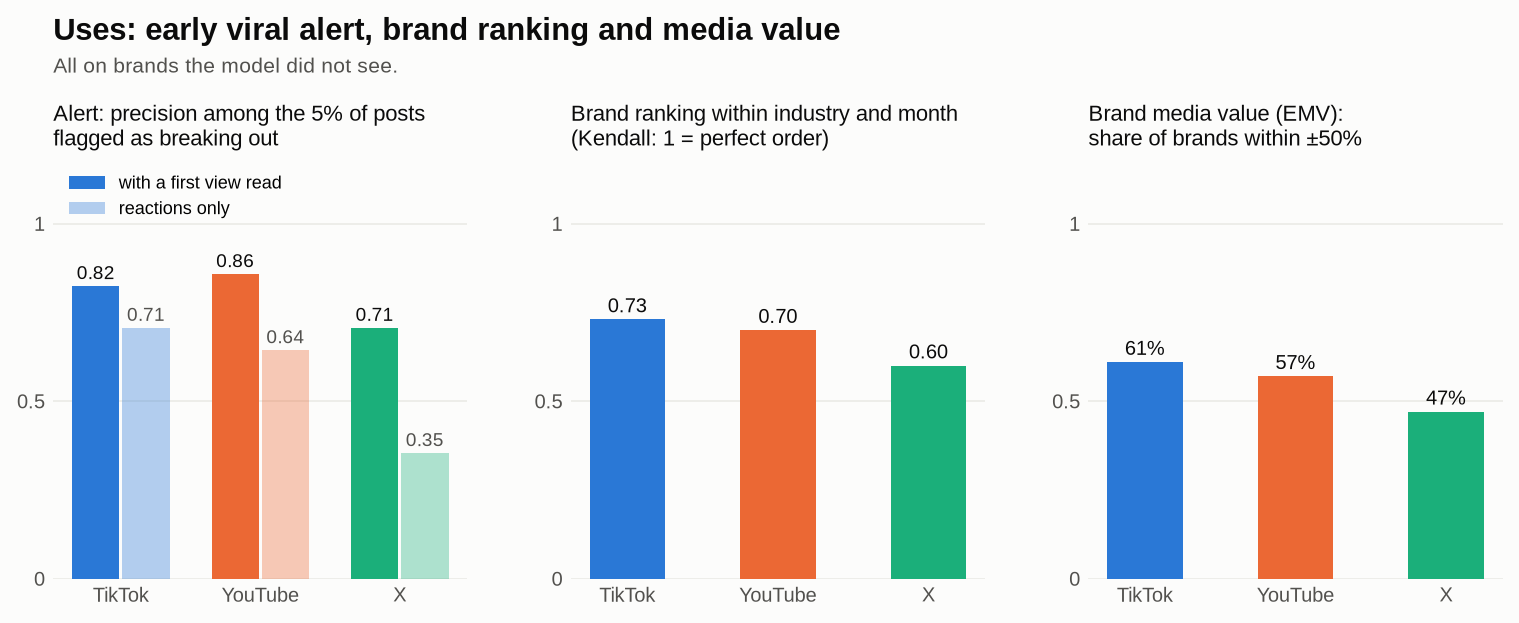
\includegraphics[width=\textwidth]{fig/preprint_side_en.png}
\caption{Applications of the estimate on TikTok, YouTube and X.
\capdet{Alert: from posts read for the first time the model flags the 5\% that will have the most views; the bar is the
share of correct flags (289--336 posts per platform, one month). Ranking: mean Kendall coefficient between the estimated
and true ordering of brands in industry--month pairs (52 / 51 / 42 pairs). EMV: views converted to money at a rate per
thousand; share of brands whose estimated EMV is within $\pm$50\% of the true one (238 / 213 / 189 brands).}}
\label{fig:side}
\end{figure}

\paragraph{Breakout alert.} With the first read of views the model flags the 5\% of posts that will break out, with
precision 0.82 / 0.86 / 0.71; reactions alone give 0.71 / 0.64 / 0.35 (Fig.~\ref{fig:side}). With three times more
alerts it catches 82--100\% of breakout posts.

\paragraph{Brand ranking.} By summing the estimated views of brands within an industry and month we recover their order
(Kendall 0.73 / 0.70 / 0.60).

\paragraph{Media value.} A brand's EMV computed from estimated views is within $\pm$50\% of the true one for 61\% /
57\% / 47\% of brands.

\paragraph{Outlying posts.} On TikTok, posts with many more views than their reactions suggest are more often promotion
(51\% against 34\%), and those with many fewer are more often spam (26\% against 13\%).
% E185, E186, E188, E184.
\todo{fill to a full page: e.g. alert precision versus number of alerts, a ranking example for one industry.}

\section{Limitations and recommendations}

The Facebook result rests on 20 brands (\x{2.9} without the three largest), and the Instagram result on 11 (\x{2.96}).
Viral posts are underestimated \x{9}--\x{14}, so brand totals are off by more than \x{2} for 29--47\% of brands. Almost
every post has a different author (2\,411 authors for 2\,491 posts on TikTok, 2\,041 for 2\,441 on YouTube, 1\,658 for
1\,803 on X), so author history cannot be used for most posts, and on Instagram the author is usually unknown. The
results describe associations, not causes. We recommend to the monitoring provider: read reactions together with views,
record missing values as missing rather than zero, take a second read of views, and keep author histories.
% E178, E180, E202.

\begin{figure}[!htb]
\centering
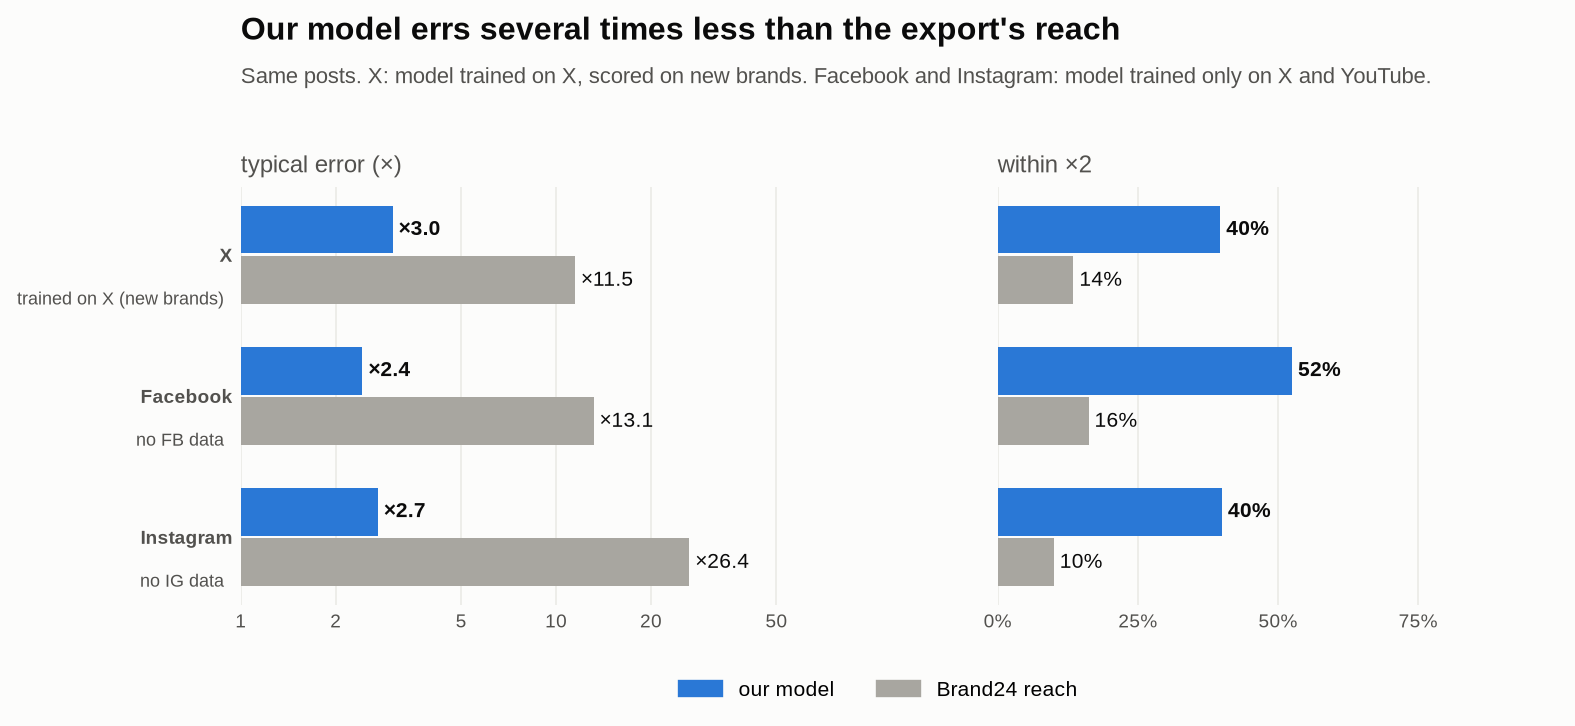
\includegraphics[width=.9\textwidth]{fig/final_compare_en.png}
\caption{Our estimate versus the reach column in the Brand24 export, on the same posts.
\capdet{Only platforms where reach is not the view count. X (1\,803 posts): model trained on X, evaluated on brands
and authors it has not seen; truth from the export. Facebook (402 videos) and Instagram (642 reels): out-of-platform
model trained only on X and YouTube, without any FB or IG post; truth from our read. Brand24 reach overestimates views
on X (74\% of posts) and Facebook (67\%), and underestimates them on Instagram (97\%).}}
\label{fig:final}
\end{figure}
% final_compare_numbers.json: X 3.03 vs 11.47; FB 2.43 vs 13.14; IG 2.72 vs 26.44.
\paragraph{Use of AI and reproducibility.} \todo{to be written by the team in their own words.} Facts to include:
AI agents (Claude Code, DeepSeek) wrote the analysis and data-reading code, ran the experiments, made the figures and a
draft of the text; language models labelled mention type and sentiment, and the labels were corrected by a team member;
the agents' session logs are in \texttt{logs/}. Every result has an experiment card, a row in the register
(\texttt{docs/en/experiments.md}, 220 entries), a script in \texttt{src/} and numbers in \texttt{data/processed/}.

\begin{thebibliography}{9}
\bibitem{tatar2014} A.~Tatar, M.~D. de~Amorim, S.~Fdida, P.~Antoniadis. A survey on predicting the popularity of web
  content. \emph{Journal of Internet Services and Applications}, 5:8, 2014.
\bibitem{shulman2016} B.~Shulman, A.~Sharma, D.~Cosley. Predictability of popularity: gaps between prediction and
  understanding. \emph{ICWSM}, 2016.
\bibitem{roy2013} S.~D. Roy, T.~Mei, W.~Zeng, S.~Li. Towards cross-domain learning for social video popularity
  prediction. \emph{IEEE Transactions on Multimedia}, 15(6), 2013.
\bibitem{catboost} L.~Prokhorenkova, G.~Gusev, A.~Vorobev, A.~V. Dorogush, A.~Gulin. CatBoost: unbiased boosting with
  categorical features. \emph{NeurIPS}, 2018.
\bibitem{romano2019} Y.~Romano, E.~Patterson, E.~Cand\`es. Conformalized quantile regression. \emph{NeurIPS}, 2019.
\end{thebibliography}

\end{document}
